\pagebreak
\section{Hiding Mechanisms of Filtering 3D Shared Surrounding Environments}
\label{sec:surrounding:hiding}

This section describes a system and a user study for hiding and showing parts of the shared social surrounding spaces on wearable AR devices. Unlike sharing for collaborative purposes, the focus of this section is on sharing between social contacts. This work extends the previous work of the Social AR Continuum by exploring how sharing the surrounding environment can vary based on the social proximity between social contacts. This work includes building a prototype for sharing a 3D captured room on a HoloLens, which enables the user to display three levels of social relationships: Intimate, Friend and Stranger, and maps them to three levels of the surrounding environment.

Previous work studied the Social AR Continuum of sharing surrounding 3D spaces by changing the level of detail of the shared 3D space based on the social proximity between viewer and sharer and focused on the viewer perspective. This work studies both the viewer and the sharer perspectives. It also allows the sharer to select which object(s) within the shared 3D space to hide or show based on the social relationship with the viewer. 

In a user study with the prototype, this work focuses on how socially connected participants felt, as well as on how they felt knowing that they were sharing more or fewer details of their surrounding environment with their social contacts. The user study found that all participant preferred having a social filter when sharing a view of their environment over having no filter. This section discusses the research findings and outlines future directions for research in sharing social surrounding spaces on wearable AR devices. 


% \subsection{Background}

% It is easy to imagine that in the future it will be possible for wearable AR systems to be used to capture and share a 3D view of the user's surroundings with hundreds or thousands of followers on a social network. However, before this becomes commonplace, many exciting research questions should be addressed. For example, 1) Would a person be comfortable with sharing a view of their real space with relative strangers? 2) Which items of the shared 3D room would the sharer want to hide or show to different levels of social proximity viewers? 3) Which hiding mechanism would the sharer prefer to use?

% This work aims to explore how wearable AR systems could share a user's surrounding room environment with social contacts as shared content and to measure how comfortable the sharer and the viewer would feel regarding privacy in different content filtering options. The key research question of this work is how do social proximity-based content filtering and its hiding mechanisms affect feelings of co-presence and the sense of privacy and comfort for both the sharer and the viewer. The hypothesis is that social proximity-based content filtering improves social presence, co-presence and the feeling of privacy. 

% It is easy to imagine that in the future it will be possible for wearable AR systems to be used to capture and share a 3D view of the user's surroundings with hundreds or thousands of followers on a social network. However, before this becomes commonplace, many exciting research questions should be addressed. For example, 1) Would a person be comfortable with sharing a view of their real space with relative strangers? 2) Which items of the shared 3D room would the sharer want to hide or show to different levels of social proximity viewers? 3) Which hiding mechanism would the sharer prefer to use?

% This work aims to explore how wearable AR systems could share a user's surrounding room environment with social contacts and to measure how comfortable the sharer and the viewer would feel regarding privacy in different interface options. 


% Previous researchers have studied the concept of "personal space" and "social bubbles" as proxemic interactions between people in different places. Greenhalgh et al. \cite{Greenhalgh1995} developed a VR teleconferencing system allowing different types of media connections (text, audio and images) between multiple users. The system was built based on the spatial model of interaction \cite{Benford1993} which defines scalability and interactions as central components of awareness consisting of an aura (total region of interaction), nimbus (region of interest and interaction) and focus of interacting objects. Sousa et al. \cite{Sousa2016} used floor projections and hand-held devices to communicate the presence of remote people, using a gradual engagement \cite{Marquardt2012} model for remote proxemics which is based on four different distances from the user; 1) personal, 2) engaged, 3) peripheral and 4) ambient.

% Jo et al. \cite{Jo2016} studied the influence of the background environment (AR vs VR) and the fidelity of the remote user's avatar representation (photo-realistic vs pre-built) on co-presence. They found that more realistic avatars had a positive impact on the feeling of co-presence between remote collaborators. Volante et al. \cite{Volante2016} also studied the effect of the visual appearance of avatars (realistic vs. stylised) on the inter-personal emotional response of participants. 

% Fuchs et al. \cite{Fuchs2014} studied telepresence via a scanned 3D environment to enable social connections with people and simulated face-to-face interactions. The remote person was scanned and reconstructed live in the local environment. They forecast that 3D telepresence is going to be more accessible when technology is more capable. Similarly, several companies are building social VR experiences in which users are represented as 3D virtual avatars, for example, High Fidelity\footnote{https://highfidelity.com/}, Sansar\footnote{https://www.sansar.com/}, Itsme3D\footnote{https://www.itsme3d.com/}) and other VR shared worlds. 

% In the social VR space, previous work implemented a variety of visual representations of self and others. For instance, virtual avatars have been used to share social experiences such as in Facebook Spaces\footnote{https://www.facebook.com/spaces} where users can meet in VR, take selfies and teleport to a 360-degree video. Virtual avatars for self and others are represented as a floating face and upper body rendered in a VR background. 

% Although there has been considerable research into social representation in VR, there has been very little research in AR. There are some challenges with AR, such as finding the best locations to fit virtual avatars in the real world, so they do not interfere with physical objects or appear suspended in mid-air. However, a social AR application can also allow people to see their social contacts while doing other tasks, i.e., users do not have to switch to an immersive VR environment to see their social contacts.

% If AR is to be used to represent contacts in social networks, there could be a large number of contacts to show. If a user has hundreds or thousands of contacts in their social network, how are these to be represented in AR? In order to answer this question, we can learn from earlier work on different ways of managing large amounts of information in AR interfaces. For example, Julier et al. showed how environmental cues such as distance, and user context could be used to filter large amounts of AR content into the most relevant information that needs to be shown\cite{Julier2002}. View management techniques can also be used to ensure that virtual objects can be easily seen in collaborative AR interfaces \cite{Hollerer2001}. Similarly, an image-based approach can be used to ensure that AR information tags do not overlap in the AR view \cite{Grasset2012}. 

% Gun Lee: The background section could be stronger. Currently, it is not clear what is the main contribution/novelty of this work compared to prior work.

\subsection{System Design and Implementation}

% An AR prototype system (Figure \ref{fig:frontier18:system}) was built to run on two Microsoft HoloLens\footnote{https://www.microsoft.com/en-us/hololens} devices that are connected to each other over WiFi. The system connects a local person (the sharer) sharing a view of their surrounding physical space to a remote person (the viewer) viewing the shared virtual room overlaid on top of their physical space.

We built an AR prototype system using the Microsoft HoloLens\footnote{https://www.microsoft.com/en-us/hololens} that connects a person (the sharer) sharing a view of their surrounding physical space to a remote person (the viewer) viewing the shared virtual room overlaid on top of their physical space. Figure \ref{fig:frontier18:system} shows the components of the system that we developed.

\begin{figure}
    \begin{center}
    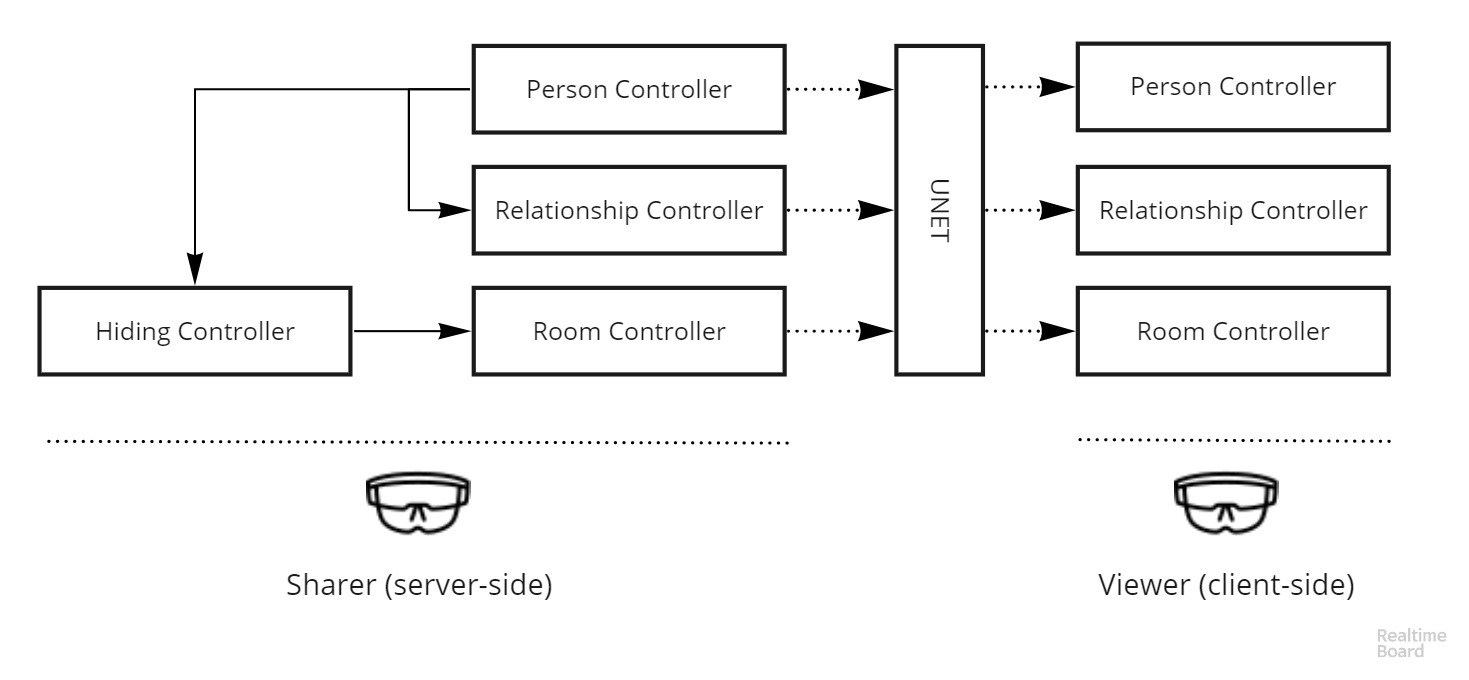
\includegraphics[width=\linewidth]{images/54-hiding-frontier18/system.jpg}
    \caption{System components representing the sharer server-side (left) sharing with the viewer client-side (right) via WiFi: 1) the avatar position and orientation, 2) the social relationship data and 3) room and hidden components data. The system is built on Unity and runs on a HoloLens.}
    \label{fig:frontier18:system}
    \end{center}
\end{figure}

% In the future, it will be possible to scan and immediately create a 3D model of the wearable AR user's surroundings. This was emulated by creating a virtual 3D room modelled to match the sharer's real room as if it had been 3D scanned.  The 3D modelling was done in Autodesk Maya\footnote{https://www.autodesk.com/education/free-software/maya} and rendered on the HoloLens display using the Unity3D\footnote{https://unity3d.com/} game engine. The avatars representing the remote people were generated using MakeHuman\footnote{http://www.makehumancommunity.org/}.

In the future, it will be possible for a person to scan and immediately create a 3D model of their surroundings. We emulate this by creating a virtual 3D room modelled to match the sharer's real room as if had been 3D scanned. The 3D model of the virtual room\footnote{Originally designed by Nikita Tuanquin} was created on Autodesk Maya\footnote{https://www.autodesk.com/education/free-software/maya} and it was visualised on the HoloLens display using the Unity3D\footnote{https://unity3d.com/} game engine. The avatars representing the remote people (who are wearing HoloLens devices) were generated using MakeHuman\footnote{http://www.makehumancommunity.org/} and rigged to a human body using Unity3D to be animated in the AR scene. When the remote person moves in real life, the avatar moves in the same direction and orientation relative to the starting position during the experiment. 

% UNet\footnote{https://docs.unity3d.com/Manual/UNet.html} was used as the high-level networking API from Unity to synchronise the state of the shared room and the remote person. The state of the remote person includes 1) the position and orientation of the virtual avatar representing the remote person, and 2) the level of detail of the avatar based on the social relationship (i.e., Stranger=half 2D image, Friend=2D image, Intimate=3D avatar). The synchronised state of the room involves changing the level of detail of the shared room depending on the social relationship as well as which part of the room is hidden by the sharer. 

We used UNET\footnote{https://docs.unity3d.com/Manual/UNet.html}, the high-level networking API in Unity, to synchronise the state of the shared room and the remote person. The state of the remote person includes 1) the position and rotation of the virtual avatar representing the remote person, and 2) the level of detail of the avatar based on their social relationship (i.e., stranger=half 2D image, friend=2D image, intimate=3D avatar). The synchronised state of the room involved changing the level of detail of the shared room depending on the social relationship as well as which part of the room is hidden by the user. The levels of details in the shared room include 1) full room where everything is shared with the viewer, 2) partial room where most items in the room are visible, but some are hidden from the viewer, and 3) limited room where most items are hidden, and only a few are visible to the viewer. These levels of detail of the shared room can be mapped onto three corresponding levels of social relationships (i.e., full room for an intimate relationship, partial room for friends, and limited room for strangers)

\subsection{User Study}

Using the prototype system, we wanted to investigate how filtering portions of the shared environment depending on the social relationship between users affects the user's perceived the social presence and sense of privacy, and also explore various methods of filtering for maintaining privacy. To do this, we conducted a user study, with 12 participants (4 female) aged (25 - 43, median=32, SD=4.96). 
We asked participants to do two tasks: test social filter and explore hiding mechanisms for filtering.

\subsubsection{Task 1 - Social Filter}

For the first task, two participants (one sharer and one viewer) were asked to observe the shared surrounding environment (a 3D model of a room) and communicate over audio about what is visible and what is hidden in the room for five minutes. The social relationship between the viewer and the sharer starts as a \textit{Stranger} relationship. The viewer then asks the sharer to upgrade the social relationship to a \textit{Friend} and then to an \textit{Intimate} relationship as a representation of a friend request on social networks. At each level of the social relationship, participants observe the changes of what is hidden and what is visible in the shared space. Two conditions are designed for this task to measure the effect of the social filter, which hides different portions and amounts of the shared surrounding space based on the social relationship. The conditions are (see Figure \ref{fig:frontier18:social-filter}): 

\begin{itemize}
\item T1C1: A shared room without a social proximity filter.
\item T1C2: A shared room with a social proximity filter. 
\end{itemize}

\begin{figure}
    \begin{center}
    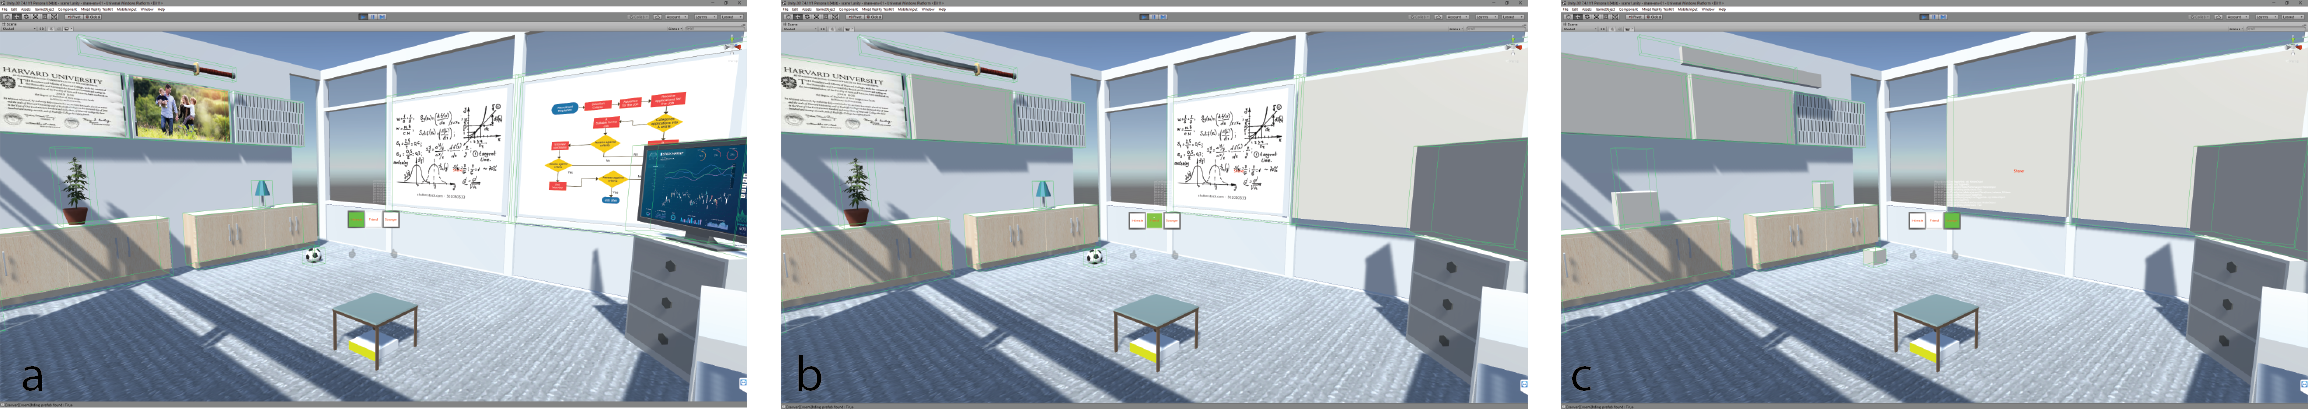
\includegraphics[width=\linewidth]{images/54-hiding-frontier18/images-02.png}
    \caption{A social filter applied to the shared room. a) In an Intimate relationship, everything is shared. b) For a Friend relationship, some sensitive items are hidden (e.g., family photo, stock market). c) While for a Stranger relationship almost everything is hidden in the room.}
    \label{fig:frontier18:social-filter}
    \end{center}
\end{figure}

\subsubsection{Task 2- Hiding Mechanism}

For the second task, the participants in the role of sharer were asked to select objects to hide in the shared environment. The sharer would aim at an object they wish to hide using a gaze indicator which appears at the centre of the view. The sharer would then use the air-tap gesture of the HoloLens to hide the selected object. The object is filtered out (or hidden) from the scene in one of three options: remove, overlay, and blur (see Figure \ref{fig:frontier18:hiding-mechanism}). These hiding mechanism options are the three conditions compared in this task and are described as the following:

\begin{itemize}
\item T2C1: Remove - objects are hidden by being removed from the viewer's scene.
\item T2C2: Overlay - objects are hidden by being overlaid with a virtual white box. 
\item T2C3: Blur - objects are hidden by appearing blurred to the viewer. 
\end{itemize}

\begin{figure}[ht]
    \begin{center}
    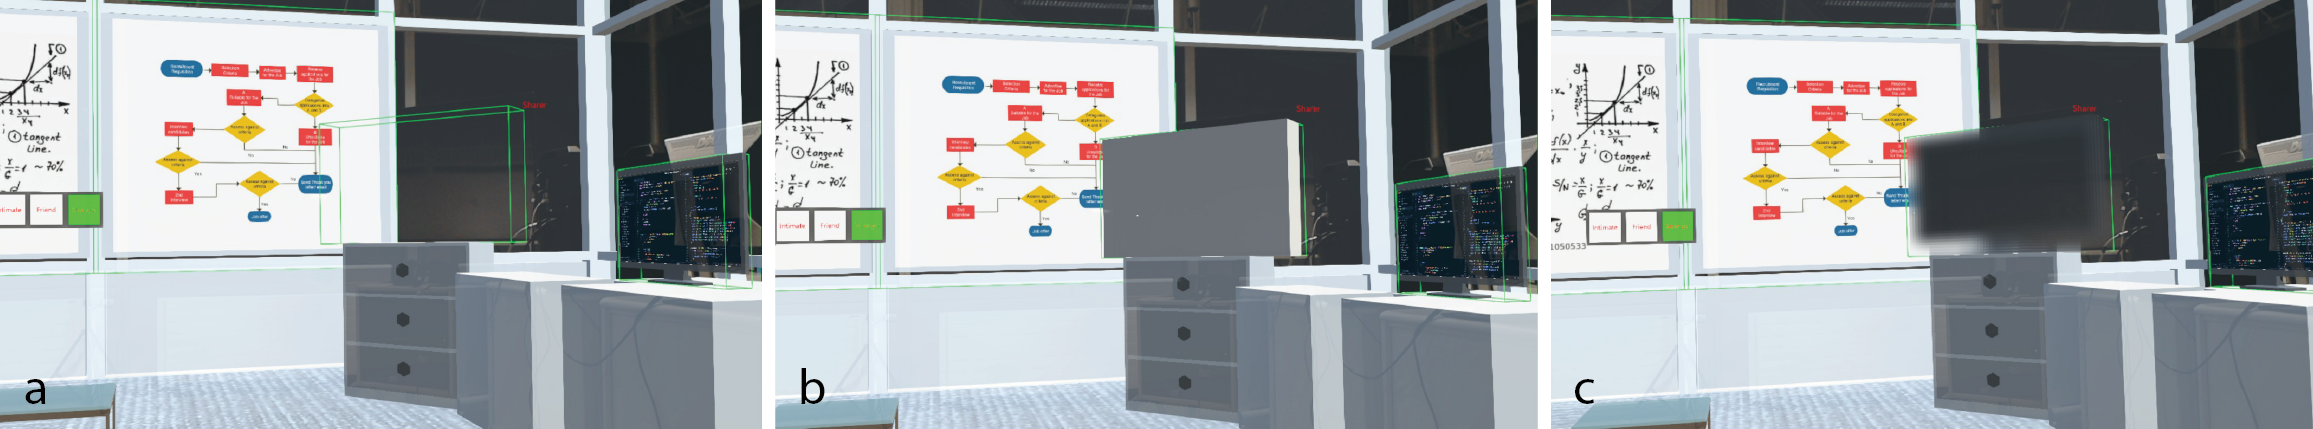
\includegraphics[width=\linewidth]{images/54-hiding-frontier18/images-01.png}
    \caption{Hiding mechanism applied on the TV screen. a) Remove, b) Overlay, c) Blur.}\label{fig:frontier18:hiding-mechanism}
    \end{center}
\end{figure}

% Each participant tried the conditions from both perspectives, a viewer and a sharer, in a counter-balanced order. Participants were asked to rate their experience after each condition. At the end of each task, participants were asked to compare the conditions to each other and rank them. 

% Figure \ref{fig:frontier18:setup} shows that the experiment was set up in two similar rooms so that the sharer was sharing their room with a remote viewer. The relative position and rotation of each user were synchronised and represented as a virtual avatar in the remote person view. The sharer could change the social relationship with the viewer (Intimate, Friend, Stranger) by using 3-buttons situated in the middle of the room. The viewer could request the relationship to change by clicking on one of the relationship buttons. Once this happened, the sharer saw the relationship request in a different colour, which they then could approve and change the social relationship.

The study was in a within-subject design; hence, each participant tried all of the conditions. Participating in pairs, each participant tried the conditions from both roles of being a viewer and a sharer by swapping the roles, each wearing a HoloLens device. The sharer saw their real physical environment overlaid with virtual green outline boxes for items to hide. The viewer saw the sharer's environment overlaid on top of the viewer space. Both the viewer and sharer saw each other as a virtual avatar which is positioned relative to where the users are inside the shared space. The rotation of the virtual avatar was mapped to the direction in which the users are looking. We asked participants to rate their experience after trying each condition. At the end of each task, we asked them to compare the conditions to each other and rank them. 


% Gun Lee: Not sure if this is necessary/meaningful as they are recruited in pairs, and randomly assigned to which role they are going to do first anyway.
Participants were recruited in pairs simulating a synchronous sharing experience. Participants were randomly assigned to play one of the roles (sharer or viewer) and then played the other role (Figure \ref{fig:frontier18:setup}). The protocol of the experiment was that each participant read an information sheet and then tried a demo of the system. Each participant went through two tasks and was asked to spend five minutes walking around the room and talking to each other over an audio link about the shared surrounding environment and to notice what is shared and what is hidden in each social relationship level. 
% Gun Lee: This paragraph is redundant, as most of the study design and procedure is already described in the previous section. Better remove, or merge into the previous section?

\begin{figure}
    \begin{center}
    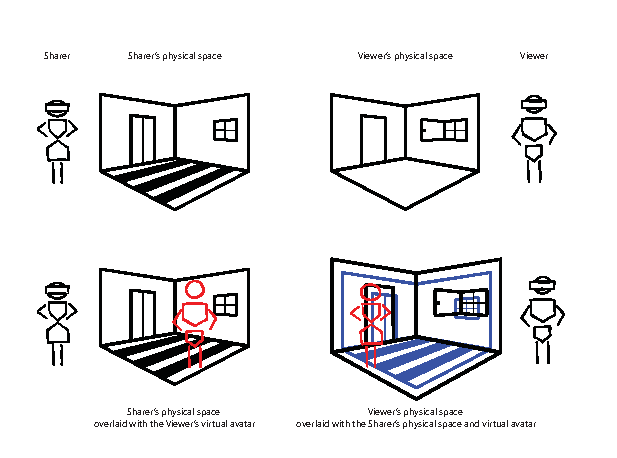
\includegraphics[width=\linewidth]{images/54-hiding-frontier18/images-23.eps}
    \caption{Experiment setup. The sharer (left) is sharing her room with the viewer (right).}
    \label{fig:frontier18:setup}
    \end{center}
\end{figure}

Figure \ref{fig:frontier18:user-study} shows the experiment set up in two similar rooms. The sharer was sharing his/her room with a remote viewer. The relative position and rotation of each user were synchronised and represented as a virtual avatar in the remote person's view. 
Both the viewer and the sharer were asked to explore different levels of social relationships. Both the sharer and the viewer were able to set the current social relationship using 3-buttons (intimate, friend, stranger) situated in the middle of the room. The current relationship level is highlighted using a green colour. The viewer could request the relationship to change by clicking on one of the relationship buttons. Once this happens, the sharer sees the relationship request as the button changing colour to a yellow colour, which then they could approve and change the social relationship.

\begin{figure}
    \begin{center}
    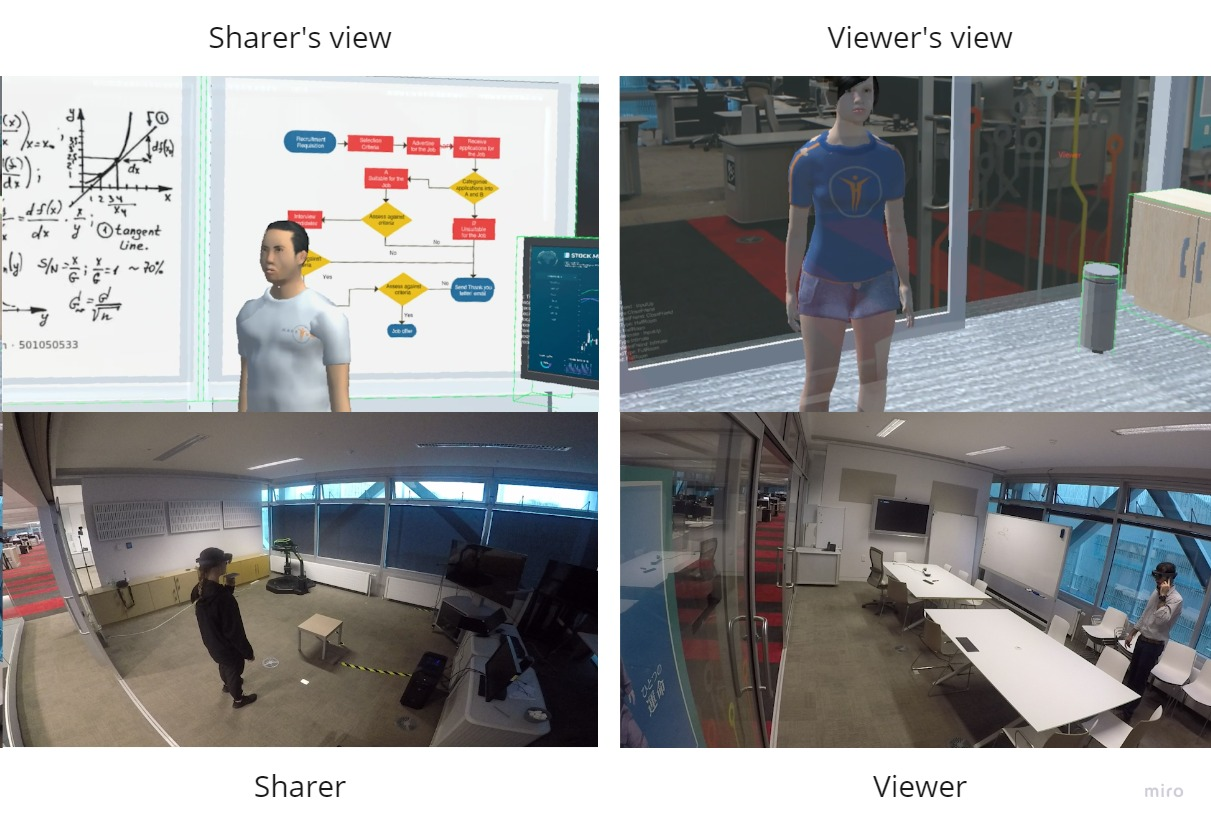
\includegraphics[width=\linewidth]{images/54-hiding-frontier18/user-study-setup.jpg}
    \caption{User study. The sharer (left) is sharing her room with the viewer (right). The viewer sees the virtual room of the sharer overlaid on top of his physical room. Each user sees the other person as a virtual avatar in their environment that has its position and orientation mapped to movements of the remote person.}
    \label{fig:frontier18:user-study}
    \end{center}
\end{figure}

After completing each task, we asked participants to answer three sets of Likert-like questionnaires: six bi-polar questions (BP) from the semantic difference measure of social presence \cite{Smith2018}, six co-presence questions (CoP) and three shared-experience questions (S) to measure the sense of privacy (see Table \ref{tab:frontier:questions}).  

\begin{table}
    \centering
    \caption{We asked participants to rate their experience on a 7-point Likert-like scale in response to the following questions: BP=bi-polar, CoP=co-presence, S=shared-experience questions}
    \begin{tabular}{ll}
BP1 &    Impersonal-Personal\\
BP2 &    Cold-Warm\\
BP3 &    Colourless-Colourful\\
BP4 &    Unsociable-Sociable\\
BP5 &    Closed-Open\\
BP6 &    Passive-Active\\
CoP1    &   I noticed my partner\\
CoP2    &   My partner noticed me\\
CoP3    &   My partner's presence was obvious to me\\
CoP4    &   My presence was obvious to my partner\\
CoP5    &   My partner caught my attention \\
CoP6    &   I caught my partner's attention\\
S1  & Uncomfortable-Comfortable\\
S2  & Insecure-Secure\\
S3  & Not-Interested-Interested\\
    \end{tabular}
    \label{tab:frontier:questions}
\end{table}

In addition to the above rating questions, participants were asked open-ended questions about the strength and weakness of each condition. We also asked them to rank the conditions for each task from the most preferred to the least preferred condition, and then explain the reason for why they chose the best and the worst condition. 

\subsection{Results}


The summarised results are shown in Figure \ref{fig:frontier18:result}. The bars indicate the mean value from all questions within the same category. The whiskers indicate standard error values. Statistically significant results are marked with *. The following subsections go into more details about the results of each question, and the statistical analysis results.

\begin{figure}
    \begin{center}
    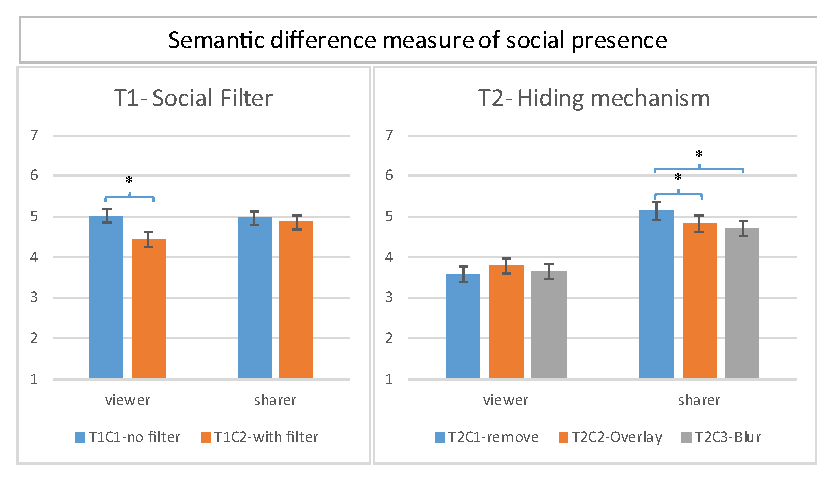
\includegraphics[width=.8\linewidth]{images/54-hiding-frontier18/images-17.eps}
    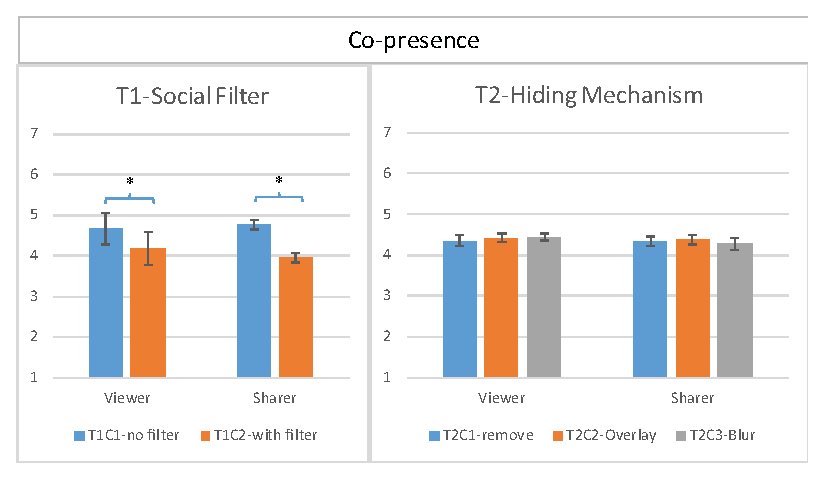
\includegraphics[width=.8\linewidth]{images/54-hiding-frontier18/images-16.eps}
    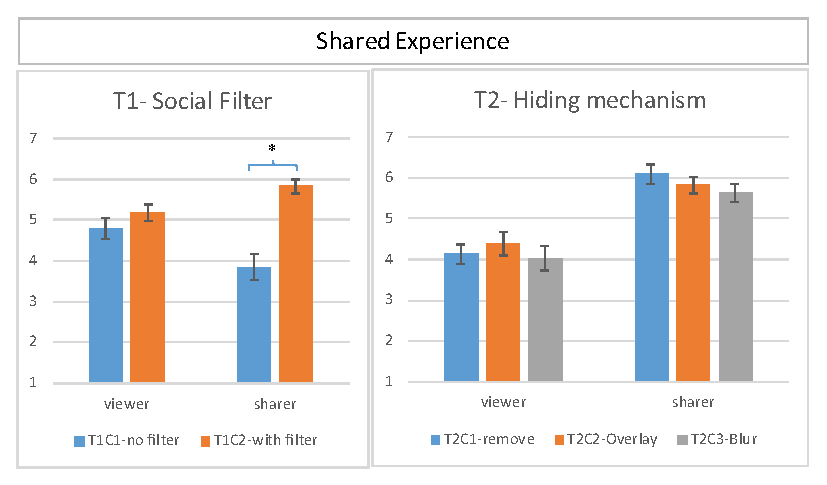
\includegraphics[width=.8\linewidth]{images/54-hiding-frontier18/images-18.eps}
    \caption{Results of semantic difference of Social Presence, co-presence and shared-experience questions: social filter and hiding mechanisms on a 7-point Likert scale as a viewer and as a sharer. *=statistically significant difference}
    \label{fig:frontier18:result}
    \end{center}
\end{figure}


\subsubsection{Task 1 - Social Filter}

For Task 1 Figure \ref{fig:frontier18:result-bipolar-filter}, comparing social filter (T1C1) to social filter (T1C2), for the semantic difference measure of social presence, a Wilcoxon signed-rank test showed that T1C2 was rated statistically significantly lower ($Z=-2.843, p=0.004$) than T1C1 as a viewer. However, there was no statistical difference as a sharer ($Z=-0.421, p=0.674$).

\begin{figure}[ht]
    \begin{center}
    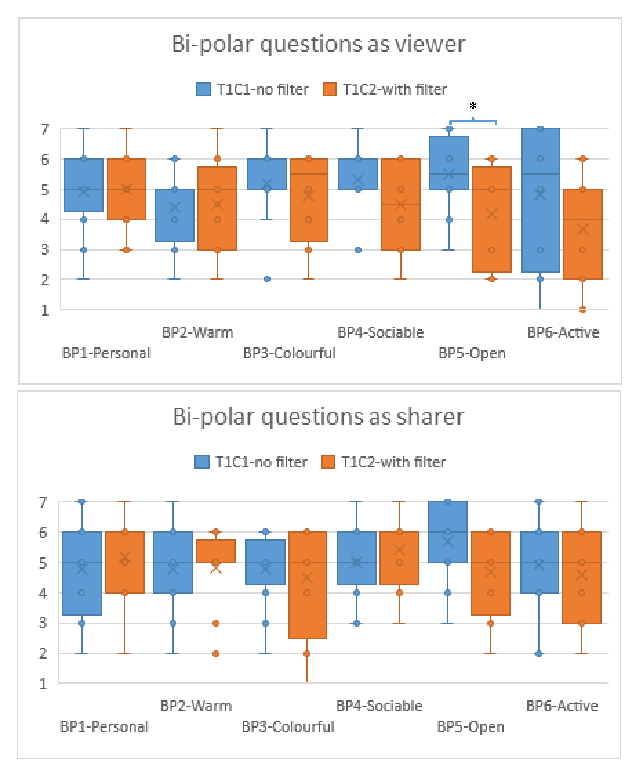
\includegraphics[width=.8\linewidth]{images/54-hiding-frontier18/images-13.eps}
    \caption{Average results of bi-polar questions for task 1 comparing two conditions: T1C1 no social filter to T1C2 with social filter. *=statistically significant result.}
    \label{fig:frontier18:result-bipolar-filter}
    \end{center}
\end{figure}

For the co-presence questionnaire (Figure \ref{fig:frontier18:result-copresence-filter}), a Wilcoxon signed-rank test showed that T1C2 was rated statistically significantly lower ($Z=-2.444, p=0.015$) than T1C1 as a viewer and as a sharer ($Z=-3.988, p<0.000$).

\begin{figure}[ht]
    \begin{center}
    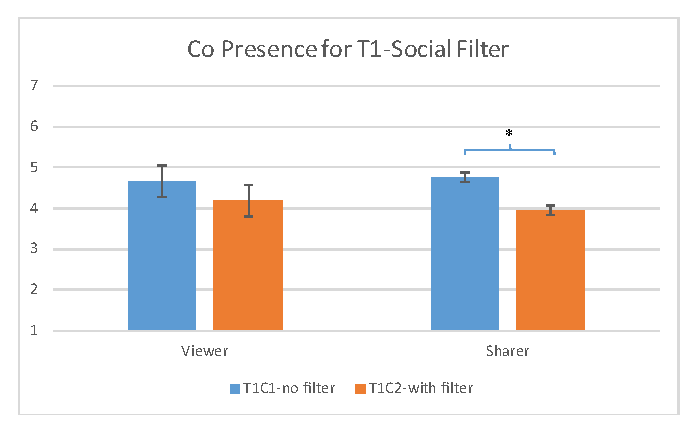
\includegraphics[width=.8\linewidth]{images/54-hiding-frontier18/images-10.eps}
    \caption{The average results of co-presence questions for task 1 comparing the two conditions: T1C1 no social filter to T1C2 with social filter. *=statistically significant result. Error bars indicate standard error.}
    \label{fig:frontier18:result-copresence-filter}
    \end{center}
\end{figure}


For the shared-experience questionnaire (Figure \ref{fig:frontier18:result-shared-experience-questions-filter}), a Wilcoxon signed-rank test showed that there was no statistical difference between T1C2 and T1C1 as a viewer ($Z=-1.689, p=0.091$); however, T1C2 was rated statistically significantly higher than T1C1 as a sharer ($Z=-4.281, p<0.000$).

\begin{figure}[ht]
    \begin{center}
    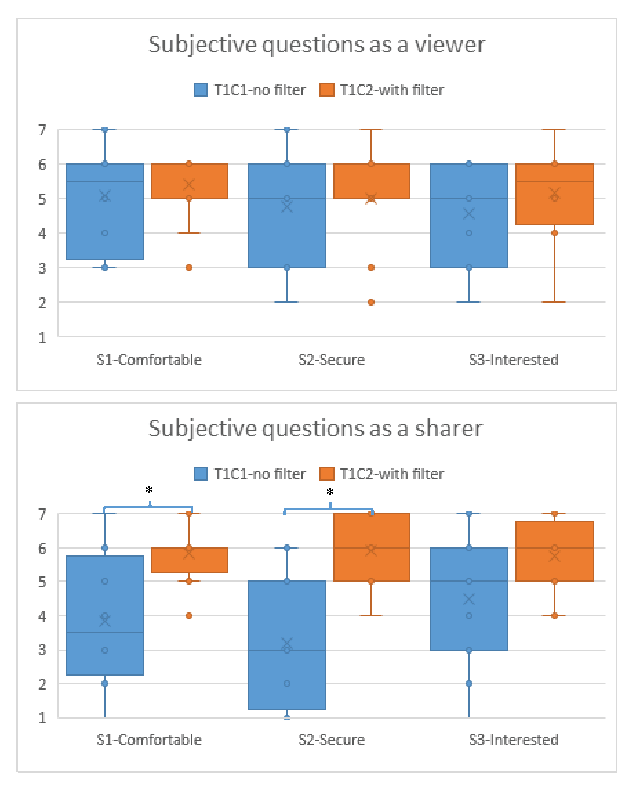
\includegraphics[width=.8\linewidth]{images/54-hiding-frontier18/images-14.eps}
    \caption{Results of shared-experience questions on social filter on a 7-point Likert scale as a viewer and as a sharer.}
    \label{fig:frontier18:result-shared-experience-questions-filter}
    \end{center}
\end{figure}

\subsubsection{Task 2 - Hiding Mechanism}

For Task 2 (Figure \ref{fig:frontier18:result-bipolar-hiding}), comparing hiding mechanism of 1) remove (T2C1), 2) overlay (T2C2) and 3) blur (T2C3), for the semantic difference measure of social presence, a Friedman test did not show statistically significant difference in the hiding mechanism as a viewer ($\chi^2(2)=3.353, p=0.187$). However, there was a statistical significance as a sharer ($\chi^2(2)=8.985, p=0.011$). Post-hoc analysis with Wilcoxon signed-rank test was conducted with a Bonferroni correction applied on the sharer results, resulting in a significance level set at $p<0.017$. There was a statistically significant difference between T2C1-remove and T2C2-overlay ($Z=-2.530, p=0.011$) and between T2C1-remove and T2C3-blur ($Z=-2.811, p=0.005$) but no statistical significant difference between T2C2-overlay and T2C3-blur ($Z=-1.073, p=0.283$).

\begin{figure}
    \begin{center}
    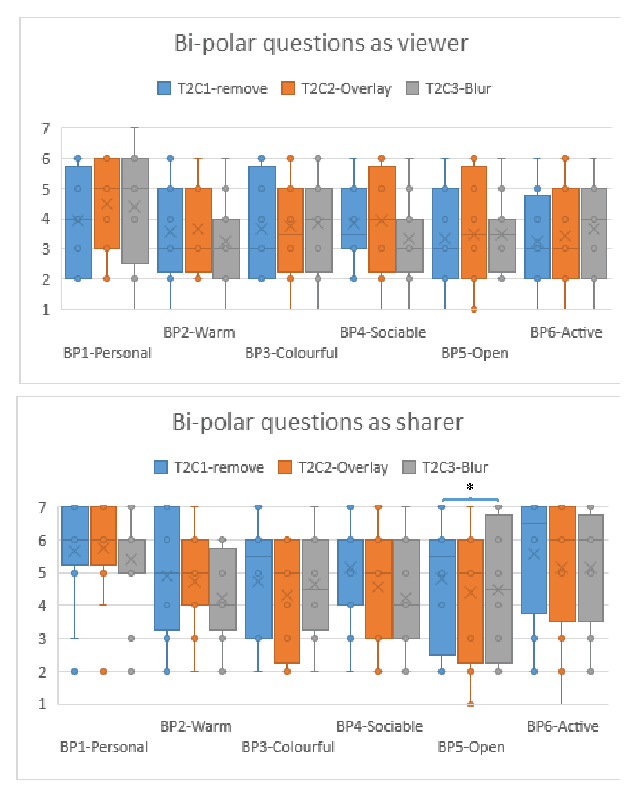
\includegraphics[width=.8\linewidth]{images/54-hiding-frontier18/images-12.eps}
    \caption{The average results of bi-polar questions for task 2 comparing three conditions of hiding mechanisms: T2C1-remove, T2C2-overlay and T2C3-blur. *=statistically significant result.}
    \label{fig:frontier18:result-bipolar-hiding}
    \end{center}
\end{figure}

For the co-presence questionnaire (Figure \ref{fig:frontier18:result-copresence-hiding}), a Friedman test did not show a statistically significant difference in the hiding mechanism as a viewer ($\chi^2(2)=0.419, p=0.811$) nor as a sharer ($\chi^2(2)=1.391, p=0.499$).

\begin{figure}
    \begin{center}
    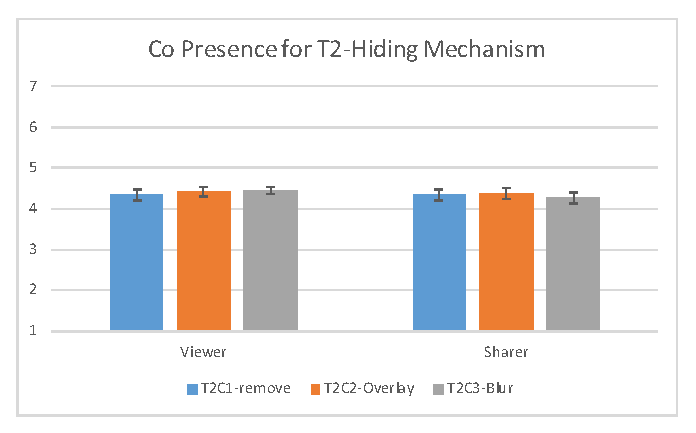
\includegraphics[width=.8\linewidth]{images/54-hiding-frontier18/images-11.eps}
    \caption{The average results of co-presence questions for task 2 comparing hiding mechanisms of three conditions: T2C1-remove, T2C2-overlay, T2C3-blur.}
    \label{fig:frontier18:result-copresence-hiding}
    \end{center}
\end{figure}

For the shared-experience questionnaire (Figure \ref{fig:frontier18:result-shared-experience-questions-hiding}), a Friedman test did not show a statistically significant difference in the hiding mechanism as a viewer ($\chi^2(2)=3.733, p=0.155$) nor as a sharer ($\chi^2(2)=5.326, p=0.070$).

\begin{figure}
    \begin{center}
    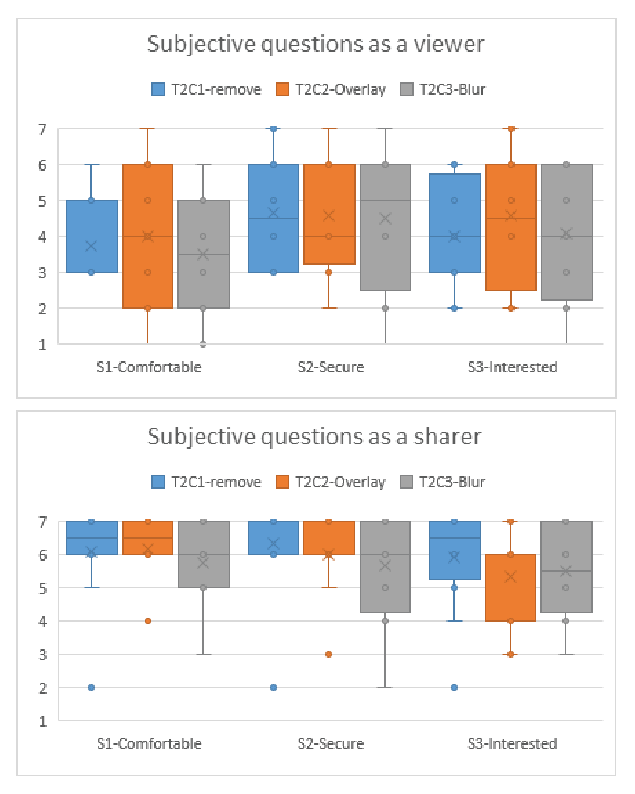
\includegraphics[width=.8\linewidth]{images/54-hiding-frontier18/images-15.eps}
    \caption{Results of shared-experience questions on hiding mechanisms on a 7-point Likert scale as a viewer and as a sharer.}
    \label{fig:frontier18:result-shared-experience-questions-hiding}
    \end{center}
\end{figure}

\subsubsection{Post-questionnaire}

In response to the ranking questions (Figure \ref{fig:frontier18:result-ranking}), all 12 participants preferred having a social filter when sharing a view of their room over having no filter (i.e., showing everything in the room to all social relationships). As for ranking the hiding mechanism (Figure \ref{fig:frontier18:result-ranking}), the most preferred option for hiding sensitive data in the room was the Remove option followed by the Overlay option, while the least preferred option was Blurring. 

\begin{figure}[h]
    \begin{center}
    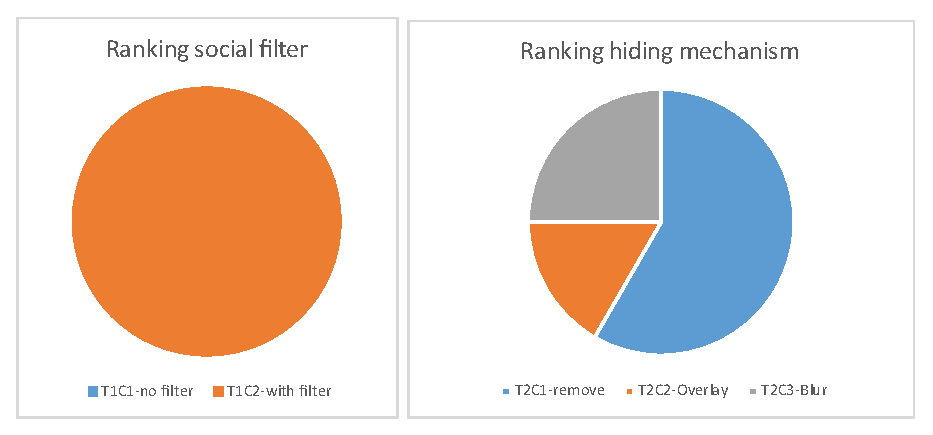
\includegraphics[width=.8\linewidth]{images/54-hiding-frontier18/images-22.eps}
    \caption{The results of the ranking conditions. Top: comparing no social filter to having social social filter in terms of choice preference. Bottom: comparing hiding mechanisms in terms of choice preference.}
    \label{fig:frontier18:result-ranking}
    \end{center}
\end{figure}

Participants were asked if there was a different mechanism for hiding objects in their shared room that they would prefer (such as replacing the hidden object with a similar but less sensitive one). About 42\% thought that replacing the object was a good idea; however, most of them raised concerns about how they may not like the additional effort needed for selecting a similar object to replace.

\subsection{Discussion}

For the first task of comparing using a social filter or not, the results showed a statically significant difference in the bi-polar rating item Close-Open of the semantic difference questions for the viewer side. Participants rated that they felt less Open as a viewer when having a social filter on. This can be explained by when no social filter is applied; it means nothing is hidden, and therefore, the participants may feel the sharing experience is more open. There was no statistically significant difference in the sharer side regarding semantic difference questions. This can be explained by when someone is sharing their room; it does not trigger an emotional response whether with or without the social filter. 
% This indicates that from the sharer's perspective, the bi-polar questions measures are not affected by having a social filter or if no social filter is applied. 

As for the co-presence questions, there was no statistically significant difference in the viewer side whether a social filter was applied or not. This indicates that the social filter does not increase or decrease social presence for the viewer. However, from the sharer's perspective, there was a statistically significant decrease in co-presence when the social filter is applied. 
% This indicates that the sharer's feeling of co-presence is decreased when a social filter is applied. This could be because hiding part of the sharer's room with some of their social contacts reduces co-presence between the sharer and viewers. 

For the shared-experience questions, there was no statistically significant effect of having a social filter on the viewer side. However, on the sharer side, having a social filter had a significantly positive effect on users feeling comfortable and feeling secure. This indicates that having a social filter will increase the sense of being comfortable and secure for the sharer. 

For the second task of comparing hiding mechanisms, there was no statistically significant difference between the mechanisms in terms of semantic difference questions, except the bi-polar rating item Close-Open for the sharer perspective. While applying a social filter felt less open in the results of task 1, the blur hiding mechanism was rated as more open compared to the overlay and remove options. There was no statistically significant difference in co-presence and shared-experience questions. 
% This indicates that the three hiding mechanisms do not affect co-presence or the feeling of comfort, security and interest. 
% Gun Lee: repetition of the previous sentence
The ranking results showed that participants preferred having a social filter. Combined with the results of shared-experience questions, the results indicate that having a social filter is essential for people to feel comfortable regarding privacy when they have to choose, but not as much when they have to go through the effort of selecting which objects to hide for each social relationship. 
% Anthony Steed: I wouldn't rely on the number of differences as a comparator.
% Anthony Steed: Use the differences in types of difference.

% \subsection{Future Work}

Future work includes allowing users to customise their room so that they feel more attached to the space they are sharing. In this user study, the sharer was hiding objects in the room while the viewer was observing the shared room at the same time. In the future, a study can be done to test if hiding before the viewer is connected would affect the sense of co-presence or the feeling of being comfortable with sharing. Additionally, this study was limited to two participants. Future studies could look into multiple (more than two) participants each are viewing and sharing with different social proximity with different people. This will be interesting to observe the group effect on sharing social experiences and to test a different way of filtering shared surrounding environments. 

% I would focus on things that extend your result.

\subsection{Conclusions}

This work described a prototype of AR social sharing experience built on a HoloLens to share a user's 3D surrounding environment with social contacts. The prototype simulates a future wearable AR social networking application. The goal of the prototype was to explore how users would be willing to share views of their surroundings with remote people with different social relationships. 

Users were allowed to choose which part of the room to hide or show to different social groups (intimate, friends, strangers). A user study was run to test the effect of using a social filter on co-presence and the feeling of privacy from both sides as a sharer and a viewer. Results showed that all participants preferred having a social filter, although it causes the feeling of being less open on the viewer side, and of lower co-presence on the sharer side. However, having a social filter had a positive effect on feeling more comfort and security on the sharer side. Results also showed that participants felt being more open when using the blur hiding mechanism compared to others, such as remove or overlay. 
